% This text is proprietary.
% It's a part of presentation made by myself.
% It may not used commercial.
% The noncommercial use such as private and study is free
% Nov. 2006
% Author: Sascha Frank 
% University Freiburg 
% www.informatik.uni-freiburg.de/~frank/
%
% additional usepackage{beamerthemeshadow} is used
%  
%  \beamersetuncovermixins{\opaqueness<1>{25}}{\opaqueness<2->{15}}
%  with this the elements which were coming soon were only hinted
\documentclass{beamer}
%\usepackage{beamerthemesplit}
\usepackage{asymptote}
\usepackage[update,prepend]{epstopdf}
\usepackage{subfigure}
%\usepackage{cite}
%\usepackage[cmex10]{amsmath}
\usepackage{amsfonts}
\usepackage{url}
\usepackage{pgf}
\usepackage{tikz}
\usetikzlibrary{arrows,chains,matrix,positioning,scopes}
%
\makeatletter
\tikzset{join/.code=\tikzset{after node path={%
\ifx\tikzchainprevious\pgfutil@empty\else(\tikzchainprevious)%
edge[every join]#1(\tikzchaincurrent)\fi}}}
\makeatother
%
\tikzset{>=stealth',every on chain/.append style={join},
         every join/.style={->}}
\tikzstyle{labeled}=[execute at begin node=$\scriptstyle,
   execute at end node=$]
\usepackage[style=ieee]{biblatex}
\addbibresource{presentation}
%\ExecuteBibliographyOptions{numeric-comp}

\usetheme{Luebeck}
\usecolortheme{lily}
\title{Image Processing}  
\author{Dr. Travis W. Axtell \\ \emph{travis.axtell@gmail.com}}
\institute{Mentor for FRC Team 612 --- Chantilly, VA \\ 
\quad\quad\quad\, FRC Team 
2035 --- 
Carmel, CA \\ \quad\quad\quad\quad\quad\quad FRC Team 5104 --- Pacific Grove, 
CA}
\date{\today} 

\addtobeamertemplate{footnote}{}{\vspace{2ex}}

\setbeamercolor{block title}{use=structure,fg=white,bg=blue!75!black}
\setbeamercolor{block body}{use=structure,fg=black,bg=black!20!white}
\setbeamertemplate{blocks}[rounded][shadow=true]
%\setbeamertemplate{blocks}

\begin{document}

\frame{\titlepage} 

\frame{\frametitle{Table of contents}\tableofcontents} 


\section{Introduction} 
\subsection{Formats}
\frame{ 
\frametitle{Modern file formats of interest}
Raster
\begin{itemize}
\item JPEG (JPG)
\item PNG
\item WEBP
\item GIF
\end{itemize}

Vector
\begin{itemize}
\item SVG
\item PDF
\end{itemize}

There are benefits to each format.  These notes discuss raster images.
}
%\begin{figure}
%	\includegraphics[scale=0.4]{SMT}
%	\caption{3-meter Segmented Mirror Telescope housed at Naval Postgraduate 
%School}
%\end{figure}
%}

\subsection{Definitions}
\frame{\frametitle{Raster Image Definitions}
\begin{columns}
\begin{column}{0.65\textwidth}
\begin{itemize}
\item A \underline{Scene}: $I(x,y)$ in continuous, physical coordinates $x$ and 
$y$.
\item An \underline{Image}: $I[n_1, n_2]$
of dimensions $N_1 \times N_2$ (width $\times$ height), where $n_1 \in \{1, 2, 
\dots, N_1 \}$
and $n_2\in \{1, \dots, N_2\}$ are all integers.
\begin{block}{Sampling}
$I[n_1, n_2] \equiv  I(n_1 \Delta x, n_2 \Delta y)$ \\
The image contains \underline{samples} of the scene.
\end{block}
\item A \underline{Pixel} resides at every $[n_1, n_2]$ index.  
%This grid follows the left-handed coordinate system convention.
\end{itemize}
\end{column}
\begin{column}{0.35\textwidth}
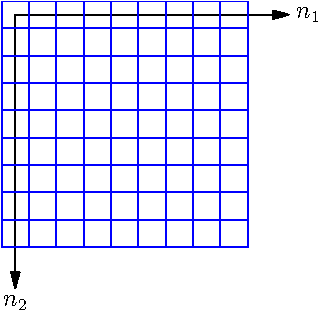
\includegraphics[width=0.9\textwidth]{coordinateframe}
\end{column}
\end{columns}
}

\frame{\frametitle{Image Processing Algorithm}
An image processing \underline{algorithm} uses the image as the input, performs 
computations, and outputs information.  Potential outputs include:
\begin{itemize}
\item Determine if an object is in the image [True/False]
\item Count objects in the image [\#]
\item Calculate the centroid of an object [$n_1, n_2$ coordinates]
\item Calculate the moment of an object
\end{itemize} 

Diagram here

This information can be used for other purposes, such as \underline{control} of 
a robot.
}

\subsection{Pixels}

\frame{\frametitle{Pixels}
Recall: $I[n_1, n_2]$ is an image that contains pixels.
\vspace{0.25cm}

How do we represent a pixel \underline{quantatively}?
}

\frame{ 
\frametitle{Pixels, round one}
%Recall: $I[n_1, n_2]$ is an image that contains pixels.
%\vspace{0.25cm}

If we make every pixel contain one number, then we can render a \underline{gray 
scale} or \underline{monochrome}\footnote{Assumes single-color light source.} 
image.

\begin{figure}
\centering
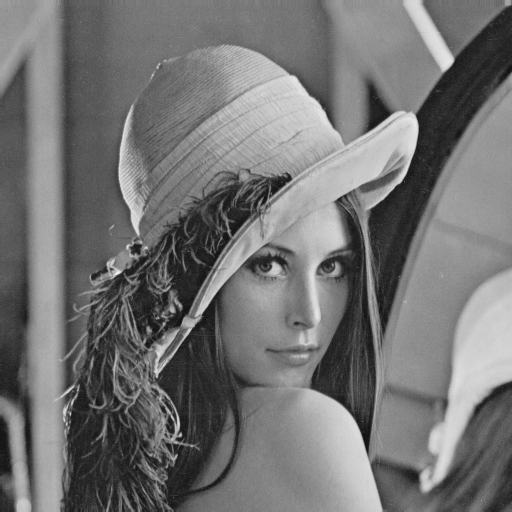
\includegraphics[scale=0.2]{LennaGray} \hspace{0.1cm}
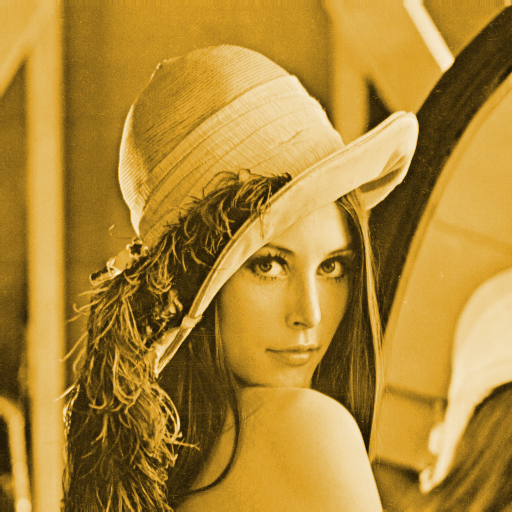
\includegraphics[scale=0.2]{LennaMono}
\caption{This image of Lena S\"{o}derberg is famous as a standard test from 
image processing literature.}
\end{figure}
}

\frame{ 
\frametitle{Pixels, round two}
%Recall: $I[n_1, n_2]$ is an image that contains pixels.
%\vspace{0.25cm}

If we make every pixel contain several numbers, then we can render a 
\underline{color} image.  Color images are stored in separate 
\underline{channels}, such as Red, Green, Blue (RGB). 

\begin{figure}
\centering
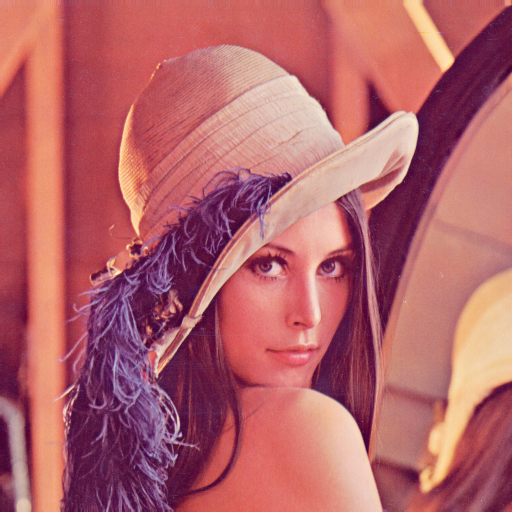
\includegraphics[scale=0.2]{Lenna}
\caption{The Lena image is composed of 3 channels.}
\end{figure}
}

\frame{ 
\frametitle{Pixels, round three}
Recall: $I[n_1, n_2]$ is an image that contains pixels.
\vspace{0.25cm}

Since \underline{digital} images $I[n_1, n_2]$ are stored on computers, pixels 
are efficiently represented as \underline{unsigned} integers. 
}

\frame{\frametitle{Pixels, review}
Recall: $I[n_1, n_2]$ is an image that contains pixels.
\vspace{0.25cm}

What \underline{information} is \underline{encoded} in pixels?

\begin{itemize}
\item Color
\item Spatial
\item Bit-depth
\item ...
\end{itemize} 
}

\section{Colors}
\frame{ 
\frametitle{Color in raster images}
Should we only use Red, Green, Blue?
\vspace{0.25cm}
\\
Paper Printers use Cyan, Magenta, Yellow, and Black (or Key) -- CMYK
\vspace{0.25cm}
\\
Computer vision uses Hue, Saturation, Lightness or Value (HSL, HSV)
\vspace{0.5cm}
\\
Why are there multiple \underline{color models}?
}

%\frame{ 
%\frametitle{Human Vision}
%\begin{figure}
%	\includegraphics[scale=0.6]{adaptiveglasses}
%\end{figure}
%}
%
%\frame{ 
%\frametitle{Comparison}
%\begin{columns}
%\begin{column}{0.65\textwidth}
%A\\B
%\end{column}
%\begin{column}{0.35\textwidth}
%\pgfputat{\pgfxy(0,0)}{\pgfbox[left,top]{\includegraphics[width=\textwidth]{DM}}}
%\end{column}
%\end{columns}
%}

%\subsection{Atmospheric Parameters}
%\frame{ 
%\frametitle{Fried's parameter}
%\begin{equation}
%r_0 = \left [ 0.423 \, k^2 \, \sec \zeta \int_{\mathrm{Path}} C_n^2(z) \, dz 
%\right ]^{-3/5}
%\end{equation}
%\begin{enumerate}
%\item 10 cm for average seeing sites
%\item 20-30 cm for best seeing sites
%\item Without AO, telescopes larger than $r_0$ in diameter have same 
%resolution as telescope of $r_0$ diameter!
%\end{enumerate}
%}
%
%\frame{ 
%\frametitle{Greenwood Frequency}
%\begin{equation}
%f_{\mathrm G} = 2.31 \, \lambda^{-6/5} \left[ \sec \zeta \int_{\mathrm{Path}} 
%C_n^2(z) \, v_{\mathrm{Wind}}(z)^{5/3} \, dz \right]^{3/5}
%\end{equation}
%\begin{enumerate}
%\item Minimum bandwidth $f_G$ required for optimal correction
%\item Faster winds $\Rightarrow$ Higher frequency correction required
%\end{enumerate}
%}
%
%%\frame{ 
%%\frametitle{Other named Constants}
%%\begin{enumerate}
%%\item Kolmorgorov Turbulence
%%\item Tyler Atmospheric Seeing Time Constant
%%\end{enumerate}
%%}
%
%
%
%
%\subsection{Diagrams}
%\frame{ 
%\frametitle{Adaptive Optics System Diagram}
%\begin{figure}
%	\includegraphics[scale=0.4]{AOsystem}
%\end{figure}
%}
%
%\frame{ 
%\frametitle{Wavefront phase composition - Zernike Basis}
%\begin{figure}
%	\includegraphics[scale=0.4]{Zernike}
%\end{figure}
%}
%
%\frame{ 
%\frametitle{Shack-Hartmann Diagram}
%\begin{figure}
%	\includegraphics[scale=0.8]{SHoverview}
%\end{figure}
%}
%
%\frame{ 
%\frametitle{Shack-Hartmann Sensor Quadcell}
%\begin{figure}
%	\includegraphics[scale=0.6]{quadcell}
%\end{figure}
%\begin{enumerate}
%\item Want at least 4 pixels per dot.
%\item More pixels per dot has increased photon shot noise, which is a problem 
%for low-SNR dim targets.
%\end{enumerate}
%}
%
%\frame{ 
%\frametitle{Shack-Hartmann Sensor Fried Geometry}
%\begin{figure}
%	\include{sh}
%\end{figure}
%\footnotesize
%\begin{subequations}
%\label{eq:sxAndsyForFried}
%\begin{align}
%s_x[m,n]& = \frac{1}{2}(b-a+d-c)  \\
%s_y[m,n]& = \frac{1}{2}(c-a+d-b) 
%\end{align}
%\end{subequations}
%}
%
%
%\frame{ 
%\frametitle{Deformable Mirror}
%\begin{figure}
%	\includegraphics[scale=0.4]{DM}
%\end{figure}
%}
%
%\frame{ 
%\frametitle{Segmented Deformable Mirror}
%\begin{figure}
%	\includegraphics[scale=0.4]{DM2}
%\end{figure}
%}
%
%\frame{ 
%\frametitle{Segmented Deformable Mirror - Phasing issue}
%\begin{figure}
%	\includegraphics[scale=0.4]{DM2bad}
%\end{figure}
%}
%
%\section{My Research Direction}
%\subsection{Introduction}
%\frame{\frametitle{Introduction} 
%\begin{itemize}
%\item Adaptive Optics systems require fast computation
%\item Large Multi-Input Multi-Output Systems scaling an issue
%\item Any techniques to decrease processing time improves control bandwidth.
%\item SMT control problem based on structural dynamics rather than atmosphere.
%\end{itemize}
%}
%
%\subsection{Phase Reconstruction}
%\frame{\frametitle{Phase Reconstruction} 
%Choice of solving technique to determine phase:
%\begin{itemize}
%\item Zonal or orthogonal Modal equations in Linear Algebra \\
%Assume $s = M y$ \\
%Solve $\hat{y} = M^{\dagger} s$ 
%\item Fourier Transform
%\item Wavelets
%\item Many more, including iterative, etc.
%\end{itemize}
%}
%
%\frame{ 
%\frametitle{Wavelet decomposition}
%\begin{figure}
%    \includegraphics[scale=0.65]{waveletimage}
%\end{figure}
%}
%
%\frame{ 
%\frametitle{Wavelet reconstruction - Square}
%\begin{figure}
%    \includegraphics[scale=0.5]{waveletrecon1}
%\end{figure}
%}
%
%\frame{ 
%\frametitle{Wavelet reconstruction - Noisy gradient}
%\begin{figure}
%    \includegraphics[scale=0.5]{waveletrecon3}
%\end{figure}
%}
%
%\frame{ 
%\frametitle{Wavelet reconstruction - Phase screen}
%\begin{figure}
%    \includegraphics[scale=0.5]{waveletrecon4}
%\end{figure}
%}
%
%\subsection{Phase Unwrapping}
%\frame{ 
%\frametitle{Phase Unwrapping}
%\begin{figure}
%    \includegraphics[scale=0.5]{phase1}
%\end{figure}
%}
%
%\frame{ 
%\frametitle{Branch Cuts}
%\begin{figure}
%    \includegraphics[scale=0.6]{branchcuts}
%\end{figure}
%}
%
%\subsection{Hexagon Lattice Control}
%
%%\section{Theory} 
%%\subsection{Hexagon lattice}
%\frame{\frametitle{Motivation for hexagon lattice}
%\begin{figure}
%	\include{segmentlensletsactuators}
%	\caption{A single segment geometry that shows the hexagon lenslets for the 
%S-H WFS and the face sheet actuators along the triangular frame.  The geometry 
%relationship between the neighboring lenslets and actuators change across the 
%mirror surface.}
%	\label{fig:sla}
%\end{figure}
%}
%
%\frame{\frametitle{Hexagon basis vectors}
%\begin{subequations}
%\begin{align}
%\mathbf{u_1}& =\begin{bmatrix}
%h \\ 0
%\end{bmatrix}\\
%\mathbf{u_2}& =\begin{bmatrix}
%h/2 \\ \sqrt{3} h/2
%\end{bmatrix}
%\end{align}
%\end{subequations}
%
%\begin{figure}
%	\include{basisvectors}
%	\label{fig:basisvectors}
%\end{figure}
%}
%%
%%\frame{\frametitle{Fried Geometry for wavefront sensors}
%%Hexagon lattice has an impact on Fried Geometry 
%%\footfullcite{fried_least-square_1977} definitions.
%%}
%%
%%\frame{
%%\begin{figure}
%%	\centering
%%	\include{lensletphasepoints}
%%	\label{fig:lpp}
%%\end{figure}
%%\begin{align}
%%s_{\mathbf{e_1}}[m,n] = \frac{1}{4} (& \phi[m+1,n-1]-\phi[m,n-1] \nonumber \\
%%& + 2(\phi[m+1,n]-\phi[m-1,n]) \nonumber \\
%%& + \phi[m,n+1]-\phi[m-1,n+1]) \label{eq:se1ForFried}
%%\end{align}
%%}
%%
%%\frame{
%%\begin{figure}
%%	\centering
%%	\include{lensletphasepoints}
%%\end{figure}
%%\begin{align}
%%s_{\mathbf{e_2}}[m,n] = \frac{1}{2} (& \phi[m+1,n]-\phi[m,n-1] \nonumber \\
%%& + \phi[m,n+1]-\phi[m-1,n])  \label{eq:se2ForFried}
%%\end{align}
%%}
%%
%%\frame{
%%\begin{figure}
%%	\centering
%%	\include{lensletphasepoints}
%%\end{figure}
%%\begin{align}
%%s_{\mathbf{e_3}}[m,n] = \frac{1}{4} (& \phi[m+1,n]-\phi[m+1,n-1] \nonumber \\
%%& + 2(\phi[m,n+1]-\phi[m,n-1]) \nonumber \\ 
%%& + \phi[m-1,n+1]-\phi[m-1,n]) \label{eq:se3ForFried}
%%\end{align}
%%}
%%
%%\frame{
%%\begin{figure}
%%	\centering
%%	\include{lensletphasepoints}
%%\end{figure}
%%\begin{align}
%%s_{\mathbf{e_4}}[m,n] = \frac{1}{2} (& \phi[m,n+1]-\phi[m+1,n-1] \nonumber \\
%%& + \phi[m-1,n+1]-\phi[m,n-1])  \label{eq:se4ForFried}
%%\end{align}
%%}
%%
%%\frame{
%%\begin{figure}
%%	\centering
%%	\include{lensletphasepoints}
%%\end{figure}
%%\begin{align}
%%s_{\mathbf{e_5}}[m,n] = \frac{1}{4} (& \phi[m,n+1]-\phi[m+1,n] \nonumber \\
%%& + 2(\phi[m-1,n+1]-\phi[m+1,n-1]) \nonumber \\ 
%%& + \phi[m-1,n]-\phi[m,n-1]) \label{eq:se5ForFried}
%%\end{align}
%%}
%%
%%\frame{
%%\begin{figure}
%%	\centering
%%	\include{lensletphasepoints}
%%\end{figure}
%%\begin{align}
%%s_{\mathbf{e_6}}[m,n] = \frac{1}{2} (& \phi[m-1,n+1]-\phi[m+1,n] \nonumber \\
%%& + \phi[m-1,n]-\phi[m+1,n-1])  \label{eq:se6ForFried}
%%\end{align}
%%}
%%
%%\frame{\frametitle{Slope measurements}
%%If Shack-Hartmann Wavefront Sensor measures $s_x[m,n]$ and $s_y[m,n]$, then 
%%$s_{\mathbf{e_1}}[m,n]$, $s_{\mathbf{e_2}}[m,n]$, $s_{\mathbf{e_3}}[m,n]$, 
%%$s_{\mathbf{e_4}}[m,n]$, $s_{\mathbf{e_5}}[m,n]$, $s_{\mathbf{e_6}}[m,n]$ are 
%%all related to $s_x[m,n]$ and $s_y[m,n]$ by vector projection. \newline 
%%
%%$\Rightarrow$ Linear Algebra and Fourier techniques apply to solving for 
%%phase points.
%%}
%%
%%\subsection{Hexagon lattice DFT}
%\frame{\frametitle{Hexagon lattice DFT}
%\begin{enumerate}
%\item Possible to take hexagon lattice DFT directly, but prefer existing 
%high-speed FFT2 algorithms.
%\item Must preserve the hexagon lattice geometry in the matrix using Voronoi 
%cells\footfullcite{dudgeon_multidimensional_1984}.  
%\end{enumerate}
%}
%\frame{\frametitle{Voronoi periodicity}
%\begin{figure}
%	\centering
%	\include{Voronoi}
%	\caption{Voronoi cell periodicity is used to fill a square matrix with 
%brackets and coordinates $[x,y]$ shown.  Hexagons shown are a periodic 
%repetition of the upper left with many hexagon lattice data points (not all 
%shown).  Other symmetric arrangements are also possible.}
%	\label{fig:Voronoi}
%\end{figure}
%}
%%
%%
%%\subsection{Plant model}
%\frame{\frametitle{Single mass node connected to neighbors}
%\begin{figure}
%	\centering
%	\input{massspringdamper}
%	\caption{The Mass-Spring-Damper arrangement of a mass node $y(m,n,t)$, its 
%	neighbors and actuator $u(m,n,t)$.  The spring and damper are lumped 
%	together in the coil for concise illustration.}
%	\label{fig:msd}
%\end{figure}
%}
%%\subsubsection{Mass node equation of motion}
%\frame{\frametitle{Single mass node equation of motion}
%\footnotesize
%\begin{equation}
%\begin{split}
%\ddot{y}(m,n,t)=& -\alpha_0 \dot{y}(m,n,t) - \beta_0 y(m,n,t) + \gamma_0 
%u(m,n,t) \\
%& - \alpha_{0,1}(\dot{y}(m,n,t)-\dot{y}(m,n-1,t)) \\
%& - \alpha_{0,-1}(\dot{y}(m,n,t)-\dot{y}(m,n+1,t)) \\
%& - \alpha_{1,0}(\dot{y}(m,n,t)-\dot{y}(m-1,n,t)) \\
%& - \alpha_{-1,0}(\dot{y}(m,n,t)-\dot{y}(m+1,n,t)) \\
%& - \alpha_{-1,1}(\dot{y}(m,n,t)-\dot{y}(m+1,n-1,t)) \\
%& - \alpha_{1,-1}(\dot{y}(m,n,t)-\dot{y}(m-1,n+1,t)) \\
%& - \beta_{0,1}(y(m,n,t)-y(m,n-1,t)) \\
%& - \beta_{0,-1}(y(m,n,t)-y(m,n+1,t)) \\
%& - \beta_{1,0}(y(m,n,t)-y(m-1,n,t)) \\
%& - \beta_{-1,0}(y(m,n,t)-y(m+1,n,t)) \\
%& - \beta_{-1,1}(y(m,n,t)-y(m+1,n-1,t)) \\
%& - \beta_{1,-1}(y(m,n,t)-y(m-1,n+1,t)) 
%\end{split}
%\label{eq:SpringMass}
%\end{equation} 
%}
%%
%\frame{\frametitle{Solution}
%\begin{align}
%y(m,n,t)= \int_{-\infty}^{\infty}\Biggl[   \sum_{l_{1},l_{2}=-1}^{1} & 
%\Bigl[h(l_{1},l_{2},t)y(m-l_{1},n-l_{2},t-\tau)\Bigr] \nonumber \\
%+ & g(t)u(m,n,t-\tau) \Biggr] d\tau
%\label{eq:MirrorPlantInTime}
%\end{align}
%
%or
%
%\begin{align}
%Y(k_{1},k_{2},s)& =H(k_{1},k_{2},s)Y(k_{1},k_{2},s)+G(s)U(k_{1},k_{2},s)
%\label{eq:MirrorPlantInFFT} \\
%G(m,n,s)& =\frac{\gamma_0}{s^2+\sigma s + \rho}
%\label{eq:GTransFuncForSpringMass} \\
%H(m,n,s)& =\frac{-\alpha_{m,n}s-\beta_{m,n}}{s^2+\sigma s + \rho}
%\label{eq:HTransFuncsForSpringMass}
%\end{align}
%}
%%
%%
%%\subsection{Controller model}
%\frame{\frametitle{Controller General idea}
%\begin{itemize}
%\item Usual thinking: have one controller per actuator
%\item Rather: one controller per spatial mode of actuators
%\item Each controller influences all actuators \\ $\Rightarrow$ Fewer 
%controllers needed under sparse conditions
%\end{itemize}
%}
%%
%%\frame{\frametitle{Control law}
%%\footnotesize
%%\begin{subequations}
%%\begin{align}
%%\dot{\hat{\bar{x}}} & = \overline{F}_{k} \hat{\bar{x}} + \overline{g} 
%%\overline{u}_{k} + K_{k} (y_k - \overline {h}_{k} \hat{\bar{x}}) \\
%%\bar{u}_k & = - L_k \hat{\bar{x}}
%%\end{align}
%%\end{subequations}
%%
%%\begin{subequations}
%%\begin{align}
%%\det(sI-\overline{F}_{k} + K_{k}\overline {h}_{k})& =\Gamma(s) \nonumber \\
%%& =s^5+\gamma_1 s^4+\gamma_2 s^3+\gamma_3 s^2+\gamma_4 s+\gamma_5 \\
%%\det(sI-\overline{F}_{k} + g L_{k})& =\Delta(s) \nonumber \\
%%& =s^5+\delta_1 s^4+\delta_2 s^3+\delta_3 s^2+\delta_4 s+\delta_5. 
%%\end{align}
%%\end{subequations}
%%
%%Full details in my thesis\footfullcite{axtell_segmented_2011}.
%%}
%%
%%
%%
%%%\subsection{Sparsity}
%%%\frame{\frametitle{Compressed Sensing}
%%%CS framework exploits the signal and measurement structure such that a 
%%%system samples and compresses the information concurrently and only needs to 
%%%process on the salient information\footfullcite{duarte_structured_2011}.
%%%}
%%%
%%%\frame{\frametitle{K-Sparse}
%%%For a basis $\lbrace\psi_i\rbrace_{i=1}^N$ in $\mathbb{R}^N$ where every 
%%%signal $x \in \mathbb{R}^N$ is described by a series of coefficients 
%%%$\theta_i$, the signal is formed by $x = \sum_{i=1}^N \psi_i \theta_i$.  If 
%%%the 
%%%signal has only $K$ non-zero $\theta_i$ coefficients, where $K \ll N$, then 
%%%it 
%%%is said $x$ is \emph{K-sparse}.
%%%}
%%
%%\section{Simulation} 
%%\subsection{Simulation set up}
%%\frame{\frametitle{Simulation set up}
%%\begin{itemize}
%%\item MATLAB SIMULINK\textregistered{} model
%%\item Phase Data source from Melissa Corley  
%%code\footfullcite{Corley:PhDThesis}.
%%\item Interpolates between the lattices as needed.
%%\end{itemize}
%%}
%%
%%
%%
%
%\subsubsection{Simulation Results}
%%\subsection{No spatial frequency reduction or vibration} 
%\frame{\frametitle{Spatial frequency sparsity}
%\begin{figure}
%	\centering
%	\includegraphics[scale=0.6]{paperfigure}
%	\caption{The error energy contribution as a percentage is compared to 
%spatial frequency radius for a simulation with no vibration and its sparsity 
%is 
%apparent.}
%	\label{fig:paperfigure}
%\end{figure}
%}
%%
%%\frame{\frametitle{Simulation results}
%%\begin{figure}
%%	\centering
%%	\includegraphics[scale=0.42]{paperfiguresurfK2NoVibNoReduction}
%%	
%%\end{figure}
%%}
%
%\frame{\frametitle{Spatial frequency contribution}
%\begin{table}
%    \caption{The number of spatial mode frequencies that have an error 
%percentage contribution at least as large as stated.}
%    \label{tab:errorpercentcontribution}
%    \centering
%    \begin{tabular}{l|l|l}
%        \hline
%        \textbf{Error contribution threshold} & \textbf{One Mirror} & 
%\textbf{Six Mirrors} \\ \hline 
%        \hline
%        $\geq 1 \%$                  & 3         & 1          \\ 
%        $\geq 0.5 \%$                & 25        & 11         \\ 
%        $\geq 0.25 \%$               & 66        & 70         \\
%        $\geq 0.1 \%$                & 273       & 262        \\
%        \hline
%    \end{tabular}
%\end{table}
%}
%
%%\subsection{Reduction in spatial frequencies without vibration} 
%
%\frame{
%\frametitle{Simulation Results}
%\begin{figure}
%	\centering
%	\includegraphics[scale=0.42]{paperfiguresurfK2NoVibWithReduction}
%\end{figure}
%}
%
%%\subsection{Reduction in spatial frequencies with vibration}
%\frame{\frametitle{Simulation Results}
%\begin{figure}
%	\centering
%	\includegraphics[scale=0.42]{paperfiguresurfK2WithVibWithReduction}
%\end{figure}
%}
%%
%\section{Conclusion}
%\frame{
%\frametitle{Summary}
%\begin{itemize}
%\item AO overview, Atmosphere Turbulence
%\item System Components Diagrams
%\item Phase Reconstruction and Unwrapping
%\item Hexagon Lattice Model and Controller
%	\begin{itemize}
%	\item Spatial Modal Controller for large flexible structures
%	\item Design allows for sparsity to customize computation requirements
%	\end{itemize}
%\end{itemize}
%}
%%
%%%\begin{frame}[allowframebreaks]
%%%  \frametitle<presentation>{References}    
%%  %\bibliographystyle{numeric-comp}
%%  %\bibliography{presentation}
%%%  \begin{thebibliography}{10}    
%%%  \beamertemplatebookbibitems
%%%  \bibitem{Autor1990}
%%%    A.~Autor.
%%%    \newblock {\em Einf¸hrung in das Pr‰sentationswesen}.
%%%    \newblock Klein-Verlag, 1990.
%%%  \beamertemplatearticlebibitems
%%%  \bibitem{Jemand2000}
%%%    S.~Jemand.
%%%    \newblock On this and that.
%%%    \newblock {\em Journal of This and That}, 2(1):50--100, 2000.
%%%  \end{thebibliography}
%%%\end{frame}

\end{document}
